\chapter{Phương án thực hiện}
\label{Chapter4}

\emph{Chương này sẽ trình bày, mô tả chi tiết về các phương pháp được sử dụng để triển khai ứng dụng.}


\section{Phương pháp xây dựng ứng dụng}
Dưới đây là sơ đồ xây dựng ứng dụng chatbot:
\begin{figure}[htp]
    \centering
    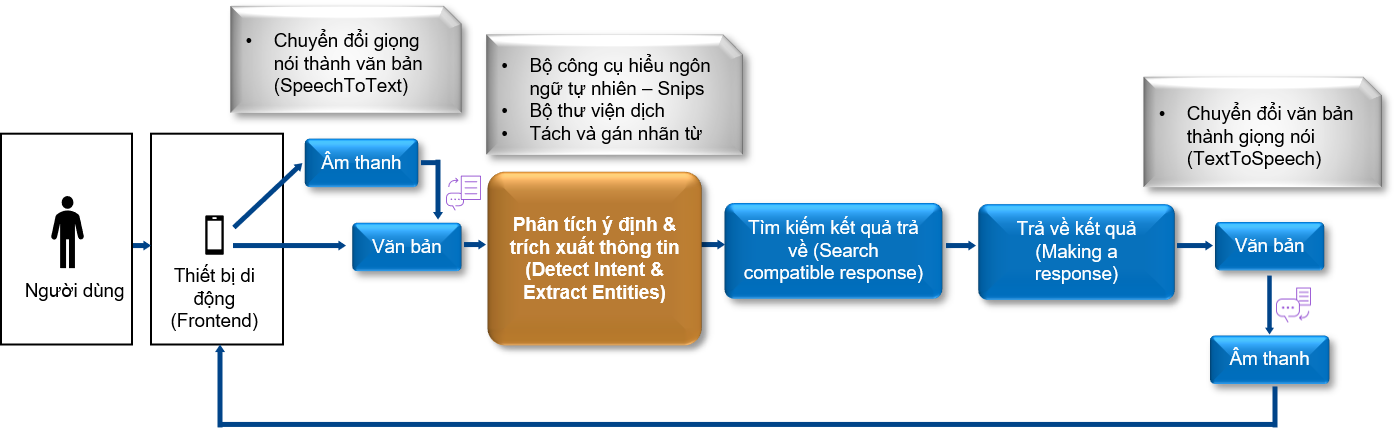
\includegraphics[width=15cm]{images/Structure-description.png}
    \caption{Sơ đồ của hệ thống chỉ đường}
    \label{fig:sodohethongchiduong}

\end{figure}

Sơ đồ này thể hiện các bước thực hiện để xây dựng ứng dụng chatbot từ dữ liêụ đầu vào đến kết quả nhận được. Các bước thực hiện được triển khai như sau:
\begin{itemize}
    \item[--] Bước 1: Khi người dùng sử dụng ứng dụng di động gửi một câu truy vấn bằng âm thanh (audio) thì ứng dụng di động sẽ chuyển giọng nói đó thành văn bản (speech to text).
    \item[--] Bước 2: Văn bản đó được gửi tới NLU engine để trích xuất ý định (intent) và các thực thể (entity).
    \item[--] Bước 3: Dựa trên ý định (intent) và thực thể (entity) nhận được, hệ thống sẽ tìm kiếm câu trả lời tương ứng và trả về cho người dùng bằng văn bản (text) và âm thanh (audio) (text to speech để chuyển văn bản thành giọng nói).
\end{itemize}
Trong phạm vi đề tài, nhóm sẽ xây dựng thành phần xác định ý định (intent),trích xuất thực thể (entity) và tìm kiếm kết quả trả lời câu hỏi sẽ sử dụng API của Google Map.

Nhóm chúng em quyết định sử dụng Snips \ac{nlu} cho việc xác định ý định (intent) và trích xuất thực thể (entity) vì:
\begin{itemize}
    \item[--] Miễn phí vì nó là opensource
    \item[--] Gọn nhẹ và dễ dàng sử dụng vì có cộng đồng lớn
    \item[--] Hiệu suất cao.
\end{itemize}

Trong hình dưới đây \ref{fig:benchmarks}, điểm F1 của cả phân loại ý định (intent) và trích xuất thực thể (entity) đã được tính toán cho một số nhà cung cấp hiểu ngôn ngữ tự nhiên (\ac{nlu}).

\begin{figure}[H]
    \centering
    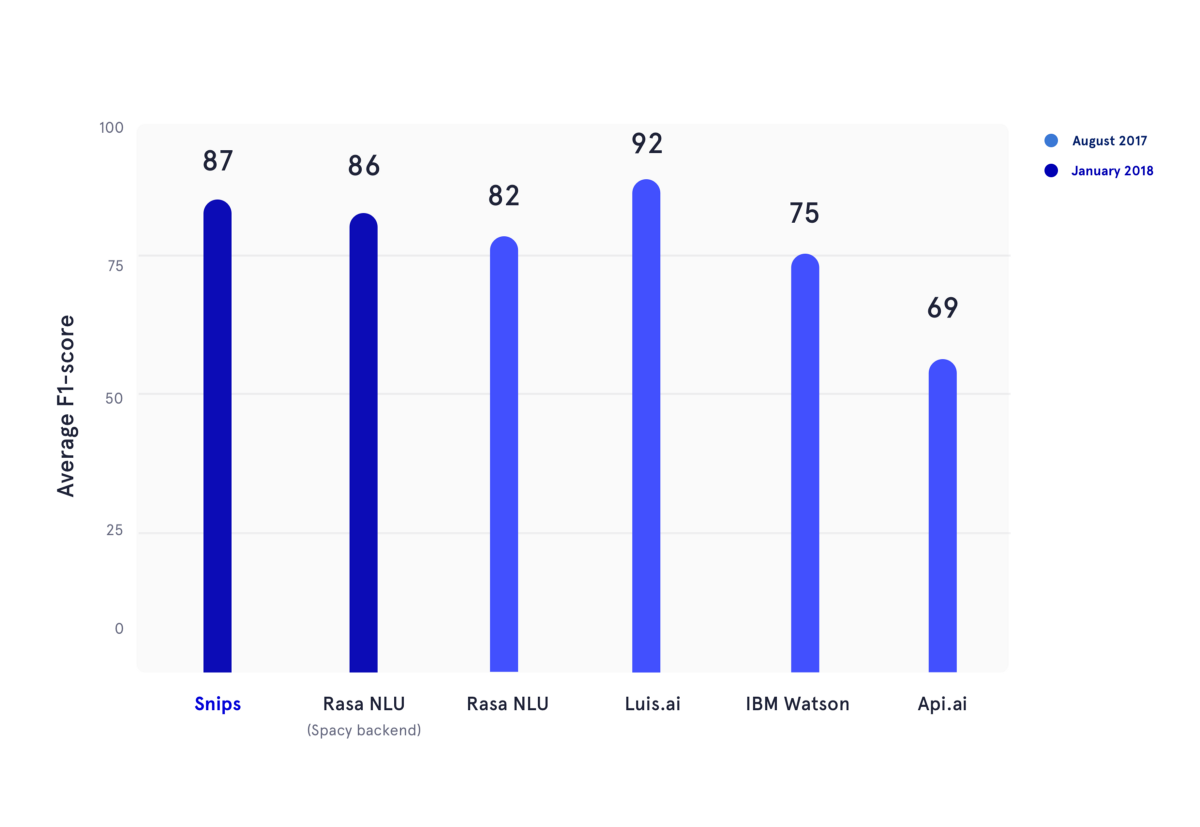
\includegraphics[width=15cm]{images/benchmarks.png}
    \caption{Bảng so sánh F1-Score giữa các nhà cung cấp hiểu ngôn ngữ tự nhiên (\ac{nlu})}
    \label{fig:benchmarks}
\end{figure}

Snips NLU là công cụ giúp hiểu ngôn ngữ tự nhiên (\ac{nlu}) mạnh mẽ, nhưng hiện tại chưa hỗ trợ tiếng Việt, mục tiêu của chúng em là xây dựng một chatbot bằng tiếng Việt. Vì thế, để có thể sử dụng được Snips NLU để trích xuất ý định (intent) và thực thể (entity), chúng em tiến hành thực hiện các bước sau đây:
\begin{itemize}
    \item[--] Bước 1: Tạo một bộ dữ liệu bằng tiếng Việt với các câu nói về chủ đề đường đi.
    \item[--] Bước 2: Chuyển hoá dữ liệu tiếng Việt sang tiếng Anh.
    \item[--] Bước 3: Dùng dữ liệu tiếng Anh được dịch sang để huấn luyện cho mô hình.
    \item[--] Bước 4: Chuyển hoá văn bản bằng tiếng Việt nhận vào sang tiếng Anh.
    \item[--] Bước 5: Đưa câu nói bằng tiếng Anh vào mô hình để trích xuất ý định (intent) và các thực thể (entity).
\end{itemize}

Về mặt dữ liệu:
\begin{itemize}
    \item[--] Định dạng bộ dữ liệu huấn luyện là ở dạng json.
\end{itemize}

\section{Chuyển hoá dữ liệu tiếng Việt sang tiếng Anh}
\subsection{Tiền xử lý dữ liệu}

\subsection{Word2word}

Với phương pháp đầu tiên, chúng em dịch bộ dữ liệu từng từ một bằng cách tách các từ theo khoảng trắng, sau đó sử dụng thư viện (word2word) để dịch từng từ này sang tiếng Anh. Ví dụ để dịch câu: "cách đi từ đại học Kinh Tế đến đại học Văn Lang".
\begin{itemize}
    \item[--] Tách câu thành từng từ riêng biệt theo khoảng trắng: ['cách', 'đi', 'từ', 'đại', 'học', 'Kinh', 'Tế', 'đến', 'đại', 'học', 'Văn', 'Lang']
    \item[--] Sử dụng thư viện word2word dịch từng từ sang tiếng Anh, ta được: ['ways', 'gone', 'word', 'Swordsman', 'learn', 'GrosDs', 'Monk', 'until', 'Swordsman', 'learn', 'Lam', 'Lang']
\end{itemize}

Sau khi dịch ta được bộ dữ liệu huấn luyện\footnote{Xem thêm về bộ huấn luyện \url{https://drive.google.com/file/d/1nfwUaNtGlk2c5oeK8b6v0lFKC2sb4uAa/view?usp=sharing}} và bộ dữ liệu kiểm thử\footnote{Xem thêm về bộ kiểm thử \url{https://drive.google.com/file/d/1Lo7Ec5CCPmH0nk3vz1LKXO1iZ2dDP9p1/view?usp=sharing}}, kết quả được minh họa như bảng \ref{fig:trainingdata_dichtungtu}.


\begin{table}[]
\begin{center}
\scalebox{0.8}{
\begin{tabular}{|l|l|}
\hline
\multicolumn{1}{|c|}{\textbf{Tiếng Việt}}                                                                & \multicolumn{1}{c|}{\textbf{Tiếng Anh}}                                                                                              \\ \hline
\begin{tabular}[c]{@{}l@{}}Đường đi từ đại học Sài Gòn \\ đến Cao đẳng Sài Gòn\end{tabular}    & \begin{tabular}[c]{@{}l@{}}Road gone word Swordsman learn Sài Gòn \\ until Higher order Sài Gòn\end{tabular}                         \\ \hline
\begin{tabular}[c]{@{}l@{}}Hướng dẫn đi từ công an Long An \\ đến ủy ban xã Bắc Hòa\end{tabular} & \begin{tabular}[c]{@{}l@{}}Direction lead gone word peacock Homeland Dragon An \\ until committee band Nazis Korea Draw\end{tabular} \\ \hline
\begin{tabular}[c]{@{}l@{}}Cách đi từ đại học Kinh Tế \\ đến đại học Văn Lang\end{tabular}       & \begin{tabular}[c]{@{}l@{}}Ways gone word Swordsman learn Gross Monk \\ until Swordsman learn Lam Lang\end{tabular}                  \\ \hline
\end{tabular}}
\end{center}
\caption{Minh họa dữ liệu trước khi dịch và sau khi dịch}
    \label{fig:trainingdata_dichtungtu}
\end{table}

\textbf{Nhận xét kết quả đạt được:}
\begin{itemize}
    \item[--] Phương pháp dịch từng từ này không khả thi bởi vì sẽ mà mất ý nghĩa của câu nói, ví dụ như câu sau: "từ Đại học Khoa học Tự nhiên đến Đại học Bách khoa đi như thế nào" được dịch thành "word Swordsman learn department learn itself course until Swordsman learn centurion department" Các thực thể địa điểm như "Đại học Khoa học Tự nhiên" được dịch thành "Swordsman learn department learn itself course", "Đại học Bách khoa" dịch thành "Swordsman learn centurion department"
    \item[--] Các thực thể (entity) cần được trích xuất đã bị dịch ra và không còn ý nghĩa nữa, không thể dùng để tìm kiếm địa điểm này trên Google map được.
\end{itemize}
\subsection{Kết hợp tách từ (word segmentation), gán nhãn (POS tagging) với thư viện dịch (word2word)}

Trong tiếng Anh, các từ được phân tách bởi dấu cách (space). Nhưng tiếng Việt thì không như thế, trong tiếng Việt có từ đơn và từ ghép, nên dấu cách không được sử dụng như một kí hiệu phân tách từ, nó chỉ có ý nghĩa phân tách các âm tiết với nhau. 

Nhận thấy được vấn đề trên. Nhóm đã tìm hiểu thêm để có thể tách các từ một cách chính xác hơn. Từ đó biết đến khái niệm tách từ (word segmentation). 

Tách từ (word segmentation) là một quát trình xử lý nhằm mục đích xác định ranh giới của các từ trong câu văn, cũng có thể hiểu đơn giản hơn là tách từ là quá trình xác định các từ đơn, từ ghép,... có trong câu.

Về vấn đề những thực thể bị dịch thành tiếng Anh làm cho nó không còn ý nghĩa nữa, nhóm em nhận thấy rằng những thực thể (entity) này chủ yếu là danh từ riêng. Nhóm em đã tìm hiểu  cách để xác định một từ thuộc từ loại nào. Từ đó chúng em biết đến khái niệm về gán nhãn từ loại (POS tagging).

Gán nhãn từ loại (POS tagging) là việc phân loại các từ trong một câu (danh từ, trạng từ, tính từ hay động từ, v.v..).

Nhóm em sử dụng thư viện VNCoreNLP để tách từ và phân loại các từ trong câu. Bảng \ref{fig:Part-Of-Speech (POS) tags} liệt kê một số loại POS tags được sử dụng phổ biến. Sau đó khi hoàn thành quá trình tách từ, chúng em sử dụng thư viện word2word để dịch những từ không thuộc từ loại danh từ và danh từ riêng. Những từ thuộc từ loại trên được giữ nguyên tiếng Việt.


\begin{table}[H]
\begin{center}
\scalebox{1}{
\begin{tabular}{|l|l|l|l|}
\hline
\multicolumn{1}{|c|}{\textbf{STT}} & \textbf{Nhãn} & \textbf{Tên}     & \multicolumn{1}{c|}{\textbf{Ví dụ}} \\ \hline
1                                  & N             & Danh từ          & Thủ đô, nhân dân, đồ đạc            \\ \hline
2                                  & Np            & Danh từ riêng    & Hồ Chí Minh, Phú Yên, Núi Đá Bia    \\ \hline
3                                  & Nc            & Danh từ chỉ loại & Con, cái, đứa                       \\ \hline
4                                  & Nu            & Danh từ đơn vị   & Lạng, cân, yến, tạ                  \\ \hline
5                                  & Ni            & Danh từ ký hiệu  & A1,  A4,  60A, 60B                  \\ \hline
6                                  & V             & Động từ          & Chơi, nhảy, ngủ                     \\ \hline
7                                  & A             & Tính từ          & Tốt, xấu, sạch, bẩn, đúng, sai      \\ \hline
8                                  & P             & Đại từ           & Tôi, chúng tôi, nó                  \\ \hline
9                                  & L             & Định từ          & Mỗi, cái, các, những                \\ \hline
10                                 & M             & Số từ            & Vài, mười, dăm, rưỡi                \\ \hline
11                                 & R             & Phó từ           & Sẽ, đang, vừa                       \\ \hline
12                                 & E             & Giới từ          & Ngoài, trong, trên, dưới            \\ \hline
\end{tabular}} 

\end{center}
\caption{Danh sách cách POS tags phổ biến}
    \label{fig:Part-Of-Speech (POS) tags}
\end{table}

Áp dụng tách từ (word segmentation) và gán nhãn từ loại (POS tagging) lên bộ dữ liệu và sử dụng thư viện word2word để dịch thì đạt được bộ dữ liệu huấn luyện\footnote{Xem thêm về bộ huấn luyện \url{https://drive.google.com/file/d/1KE6IMt7KTVu5LRQWI9b57EUgWuqBRgp_/view?usp=sharing}} và bộ dữ liệu kiểm thử\footnote{Xem thêm về bộ kiểm thử\url{https://drive.google.com/file/d/1YHs3dFAT0br8RbctmWYQtdIKQmv6j1su/view?usp=sharing}}, kết quả dịch được minh họa như hình \ref{fig:trainingdata-wordsegment}

\begin{figure}[htp]
    \centering
    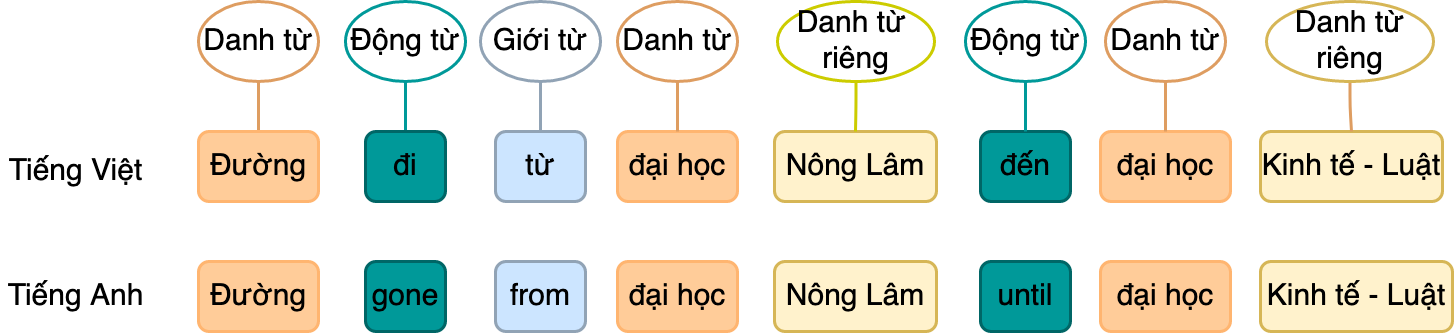
\includegraphics[width=15cm]{images/trainingdata-wordsegment.png}
    \caption{Hình ảnh minh họa dữ liệu trước khi dịch và sau khi dịch bằng phương pháp dùng word segmentation và POS tagging}
    \label{fig:trainingdata-wordsegment}
\end{figure}

\textbf{Nhận xét kết quả đạt được:}
\begin{itemize}
    \item[--] Phương pháp này nhận được kết quả tốt hơn. Nhưng vẫn có trường hợp còn chưa chính xác. Vd: Công viên giải trí Đầm Sen => Công viên entertainment Đầm Sen.
   
\end{itemize}

\subsection{Xây dựng bộ từ điển}
Để có thể xử lý tốt hơn về vấn đề ý nghĩa trong câu được dịch sang một cách chính xác hơn. Nhóm chúng em đã quyết định xây dựng mô hình so khớp dài nhất (longest matching), bằng cách xây dựng một bộ từ điển, và tìm từ dài nhất có trong bộ từ điển đó để tiến hành dịch. Bộ từ điển này nằm trong phạm vi hỏi đường nên có thể xây dựng với các từ ngữ cụ thể có trong chủ đề, từ đó việc dịch sẽ đạt hiệu quả hơn.

Trong phạm vi các câu hỏi về đường đi, chúng em đã lựa chọn dịch khoảng 100 từ và các cụm từ. Các bước để dịch được dữ liệu như sau:
\begin{itemize}
    \item[--] Bước 1: Xây dựng bộ từ điển riêng biệt về chủ đề hỏi đường đi và chuyển hoá từ ngôn ngữ tiếng Việt sang tiếng Anh.
    \item[--] Bước 2: Tìm từ dài nhất trong câu có trong bộ từ điển.
    \item[--] Bước 3: Lấy nghĩa của từ tương ứng trong từ điển.
\end{itemize}
Trong quá trình nghiên cứu, chúng em nhận thấy bước 2 là bước thật sự cần thiết để có thể tìm được từ thích hợp nhất với bộ từ điển để có kết quả tốt nhất. Dưới đây là mô tả quá trình tìm từ dài nhất có trong từ điển mà nhóm chúng em thực hiện (Xem hình Tìm từ dài nhất \ref{fig:longest-word})
\begin{itemize}
    \item[--] Input: "Đường đi từ Đại học Nông Lâm đến Ngã tư Thủ Đức""
    \item[--] Output: ["Đường đi", "từ", "Đại học Nông Lâm", "đến", "Ngã tư Thủ Đức"]
\end{itemize}
\begin{figure}[H]
    \centering
    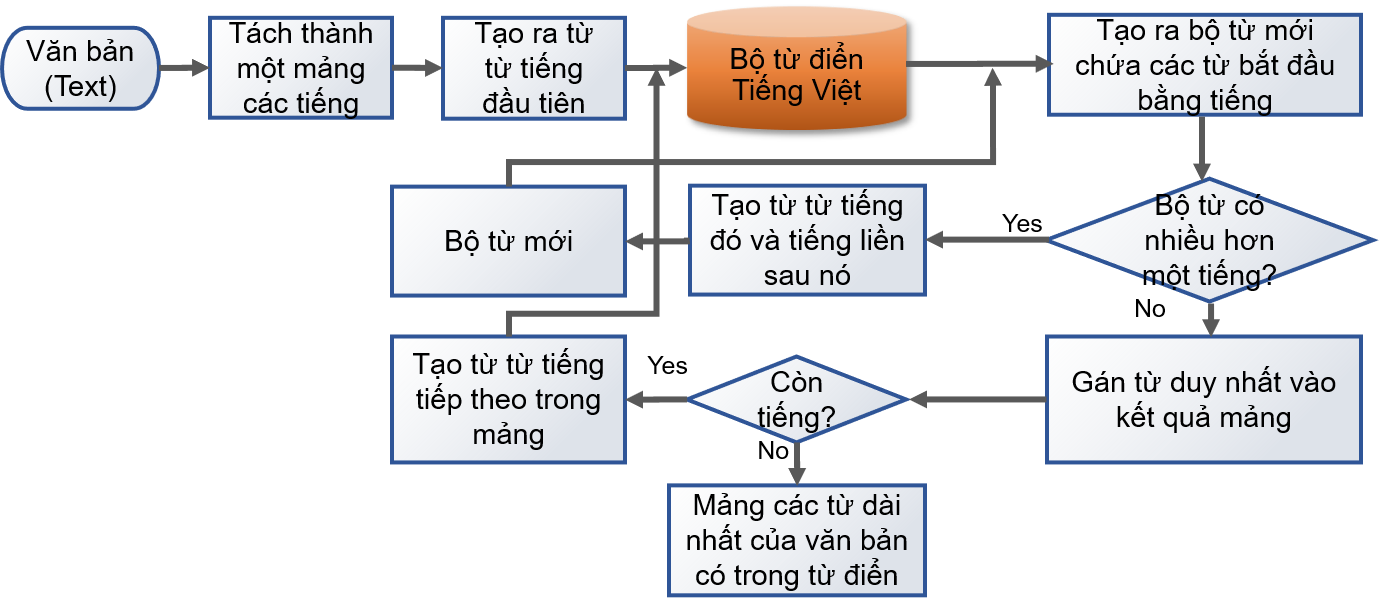
\includegraphics[width=15cm]{images/Diagram-longest-word.png}
    \caption{Tìm từ dài nhất}
    \label{fig:longest-word}
\end{figure}

Sau khi dịch ta được bộ dữ liệu huấn luyện\footnote{Xem thêm về bộ huấn luyện \url{https://drive.google.com/file/d/1VSDhjrSghKtHmQxhWfC_x-qyOKDm3YuM/view?usp=sharing}} và bộ dữ liệu kiểm thử \footnote{Xem thêm về bộ kiểm thử \url{https://drive.google.com/file/d/1S631oRroP67z6LRwGSNwkrx-22c10baJ/view?usp=sharing}}, kết quả dịch được minh họa như bảng \ref{fig:trainingdata-tudien}

\begin{table}[htp]
\begin{center}
\scalebox{1}{
\begin{tabular}{|l|l|}
\hline
\multicolumn{1}{|c|}{\textbf{Tiếng Việt}}                                                        & \multicolumn{1}{c|}{\textbf{Tiếng Anh}}                                                         \\ \hline
\begin{tabular}[c]{@{}l@{}}Đường đi từ đại học Sài Gòn \\ đến Cao đẳng Sài Gòn\end{tabular}      & \begin{tabular}[c]{@{}l@{}}Find path from đại học Sài Gòn \\ to Cao đẳng Sài Gòn\end{tabular}   \\ \hline
\begin{tabular}[c]{@{}l@{}}Hướng dẫn đi từ công an Long An \\ đến ủy ban xã Bắc Hòa\end{tabular} & \begin{tabular}[c]{@{}l@{}}Intruct go from công an Long An \\ to ủy ban xã Bắc Hòa\end{tabular} \\ \hline
\begin{tabular}[c]{@{}l@{}}Cách đi từ đại học Kinh Tế \\ đến đại học Văn Lang\end{tabular}       & \begin{tabular}[c]{@{}l@{}}Find path from đại học Kinh Tế \\ to đại học Văn Lang\end{tabular}   \\ \hline
\end{tabular}}
   \caption{Hình ảnh minh họa dữ liệu trước khi dịch và sau khi dịch bằng phương pháp xây dựng từ điển}
    \label{fig:trainingdata-tudien}
    \end{center}
\end{table}

Kết quả đạt được sau khi dùng phương pháp dịch bằng cách xây dựng bộ từ điển:
\begin{itemize}
    \item[--] Do xây dựng bộ từ điển những từ vựng trong phạm vi nhỏ - hỏi đường nên bộ dịch cho ra kết quả khá tốt, cải thiện hơn so với 2 phương pháp trước là phương pháp dịch từng từ và phương pháp dịch dùng word segmentation và POS tagging
\end{itemize}

\section{Công nghệ}

\subsection{Bộ công cụ xây dựng Fontend - Flutter}
Để xây dựng giao diện ứng dụng cho hệ thống nhóm đã tiến hành tìm hiểu nhiều công nghệ xây dựng ứng dụng di động (mobile) như React Native\footnote{Xem thêm về React Native tại đây: \url{https://reactnative.dev/}}, Xamarin\footnote{Xem thêm về Xamarin tại đây: \url{https://docs.microsoft.com/en-us/xamarin/}}, Flutter\footnote{Flutter là một bộ công cụ giao diện người dùng để xây dựng ứng dụng cho nhiều nền tảng khác nhau như web, thiết bị di động, máy tính cá nhân với cùng một mã nguồn. Xem thêm về Flutter tại đây: \url{https://flutter.dev/}}.

Nhóm quyết định chọn Flutter vì các ưu điểm sau:
\begin{itemize}
    \item[--] Flutter là công nghệ mới nhưng có cộng đồng sử dụng đông đảo và phát triển nhanh, dễ dàng tìm được hỗ trợ nếu xảy ra lỗi
    \item[--] Bộ giao diện dựng sẵn của Flutter tuân thủ đầy đủ bộ quy tắc thiết kế giao diện Material Design\footnote{Bộ quy tắc thiết kế giao diện hiện đại và phổ biến của Google. Xem thêm về Material Design tại đây: \url{https://material.io/design}}, mang đến một giao diện hiện đại cho hệ thống
    \item[--] Flutter mang đến tính năng hot reload\footnote{Tính năng cho phép những thay đổi trong mã nguồn được hiển thị gần như lập tức trên giao diện}, kết hợp với bộ giao diện dựng sẵn và trình kiểm tra lỗi dễ sử dụng giúp quá trình phát triển nhanh chóng
\end{itemize}

\subsection{Bộ công cụ hiểu ngôn ngữ tự nhiên - Snips NLU}
Snips NLU - bộ công cụ trích xuất thông tin có cấu trúc từ các câu được viết bằng ngôn ngữ tự nhiên, mã nguồn mở được viết bằng Python.
Đây là một bộ công cụ được sử dụng rộng rãi để phục vụ những nhà nghiên cứu hiểu ngôn ngữ tự nhiên (\ac{nlu}) nhằm xây dựng một hệ thống hiểu được ngôn ngữ mà con người sử dụng. Các bài báo liên quan mà nhóm tìm hiểu được sử dụng trong đề tài được thực hiện trên bộ công cụ này. Mô hình huấn luyện được nhóm tự xây dựng và sử dụng công cụ này để huấn luyện.

\begin{figure}[htp]
    \centering
    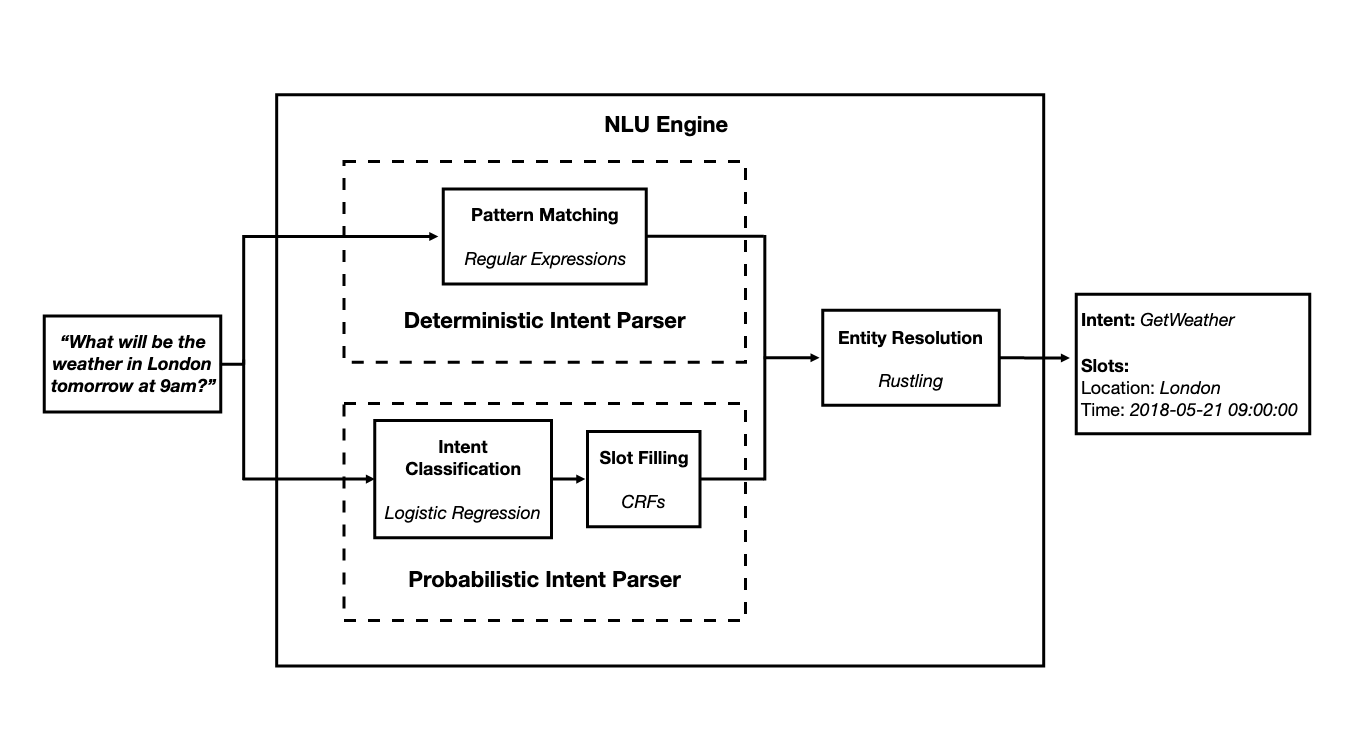
\includegraphics[width=15cm]{images/Snips-NLU.png}
    \caption{Sơ đồ hệ thống Snips NLU}
    \label{fig:snips-nlu}
\end{figure}

Có thể khái quát các luồng xử lý của snips-NLU \cite{snips-nlu} như sau:

Trung tâm của hệ thống Snips-NLU (hình \ref{fig:snips-nlu}) là NLU Engine, bản thân nó bao gồm một số thành phần sau:
\begin{itemize}
    \item Trình phân tích ý định xác định (Deterministic intent parser): Mục tiêu của trình phân tích ý định xác định là cung cấp độ mạnh mẽ và trải nghiệm có thể dự đoán được cho người dùng vì nó được đảm bảo đạt được 1.0 F1-Score trên các ví dụ đào tạo. Các truy vấn có trong dữ liệu huấn luyện được sử dụng để xây dựng các mẫu bao gồm tất cả các tổ hợp giá trị thực thể.
    \item Trình phân tích ý định xác suất (Probabilistic intent parser): Trình phân tích ý định xác suất nhằm mục đích mở rộng phân tích cú pháp vượt ra ngoài các ví dụ đào tạo và nhận ra các biến thể không xuất hiện trong dữ liệu đào tạo. Nó cung cấp sức mạnh tổng quát hóa mà trình phân tích định xác định thiếu. Thông qua hai bước intent classification (xác định ý định) and slot filling (trích xuất thực thể).
    \item Entity resolution: Phân giải thực thể giúp biến đổi các giá trị thực thể (entity) thành định dạng chuẩn ISO. Ví dụ: giá trị thực thể là "tomorrow evening" sẽ được biến đổi thành "2018-04-19 19:00:00 +00:00". Những giá trị thực thể có thể được phân giải là những thực thể được dựng sẵn (built-in entities) (numbers, ordinals, amounts with unit, date and times, durations, v.v...)
\end{itemize}

\subsection{Bộ công cụ xây dựng Backend - Flask Python}
Python ngày càng chứng minh ưu thế của mình trong việc xây dựng và triển khai nhiều loại ứng dụng khác nhau như web application, desktop application, Machine Leaning, Deep Learning,...

Để xây dựng \ac{api} cho hệ thống và thuận tiện cho việc nghiên cứu, nhóm chúng em đã tiến hành tìm hiểu nhiều framework để xây dựng trên Python như Flask\footnote{Xem thêm về Flask tại đây:\url{https://flask.palletsprojects.com}}, Django\footnote{Xem thêm về Django tại đây:\url{https://docs.djangoproject.com}}, Tornado \footnote{Xem thêm về Tornado tại đây: \url{https://www.tornadoweb.org}}, Pyramid\footnote{Xem thêm về Pyrmaid tại đây: \url{https://docs.pylonsproject.org/}}

Nhóm quyết định chọn Flask Python vì các ưu điểm sau:
\begin{itemize}
    \item[--] Đơn giản và dễ dàng sử dụng
    \item[--] Flask Python là micro web framework, không cần công cụ hoặc thư viện cụ thể, nó mang đến các chức năng tối giản nhưng có thể mở rộng cho các ứng dụng web.
    \item[--] Hỗ trợ xây dựng các \ac{api}, web services, các ứng dụng web application cỡ vừa và nhỏ.
    \item[--] Flask cung cấp rất nhiều tài liệu từ cài đặt đến thực hiện và triển khai, từ hướng dẫn nhanh đến hướng dẫn chi tiết. Nguồn tài liệu tham khảo về Flask rất phong phú giúp dễ dàng tham khảo và tìm hiểu.
\end{itemize}

Theo đánh giá năm 2020 của JetBrains Python Developers Survey\footnote{Xem thêm tại đây: \url{https://www.jetbrains.com/lp/python-developers-survey-2020/}} thì Flask hiện là framework được sử dụng rộng rãi nhất, chiếm tới 46\% thị phần.
\subsection{Google Maps API}
Google Maps API \footnote{Xem thêm về Google Maps API tại đây: \url{https://developers.google.com/maps/documentation}} là một phương pháp cho phép một website, ứng dụng B có thể sử dụng dịch vụ hoặc hiển thị nội dung của một trang web khác, ở đây là website A – Google Maps (thông qua Map API), dịch vụ bản đồ của website A (Map) sẽ được nhúng vào website B (Website cá nhân), tại trang web B có thể sử dụng những dịch vụ mà Google Maps cung cấp thông qua Google Maps API như: đường đi, đánh dấu trên bản đồ, danh sách các địa điểm muốn tìm,...

Hiện nay, các ứng dụng xây dựng trên nền tảng Google Maps như Grab, AndroidAuto,... thường sử dụng Google Maps API để nhúng bản đồ vào trang web hoặc ứng dụng thông qua nhiều cách khác nhau, chính vì vậy mà việc sử dụng API từ Google cũng khá dễ dàng. Đồng thời Map API cũng không chỉ hỗ trợ cho máy tính và website mà còn cả thiết bị di động, giúp ứng dụng hoạt động nhanh hơn và hiệu quả hơn.

Một số ứng dụng của Google Maps API :
\begin{itemize}
    \item[–-] Tính năng chỉ đường đến địa điểm cần tìm (tuyến đường tối ưu nhất cho các phương tiện và nhiều lựa chọn khác).
    \item[–-] Giúp khoanh vùng khu vực như khu đô thị hay các khu vực mà bạn muốn.
    \item[–-] Có thể theo dõi tình hình giao thông, lưu lượng phương tiện tại các khu vực,... và có giải pháp hợp lý.
\end{itemize}
